%!TEX root = kotov.tex
\section{Task 2}
\begin{task}
    Даны массив из $n$ чисел и $m$ чисел $p_1, p_2, \ldots, p_m$, нужно за $\O(n\log m + m)$ для каждого $i$ найти $p_i$-ую порядковую статистику.
\end{task}

\begin{solution}
    Так как числа $\{p_i\}$ натуральные по своему смыслу, то мы можем за $\O(n + m)$ отсортировать их с помощью \texttt{CountSort}. Разобьем этот массив пополам, то есть рассмотрим массив $[p_1,\ldots,p_{m/2},\ldots,p_m]$. Найдем соответствующую $p_{m/2}$-ую порядковую статистику (обзовем массив из $n$ числе как $\vec{x}$). Тогда исходный массив разделится на части $[x_1, \ldots, x_{p_{m/2}}, \ldots, x_n]$, с элементами слева от $x_{p_{m/2}}$ меньше, чем этот элемент, а справа --- больше. Теперь рекурсивно запустим поиск такой же соответствующей статистики для $[p_1, \ldots, p_{m/2-1}]$ и $[x_1, \ldots, x_{p_{m/2-1}}]$ и для $[p_{m/2+1},\ldots, p_m]$ и $[x_{p_{m/2+1}},\ldots,x_n]$:
    \begin{figure}[H]
        \centering
        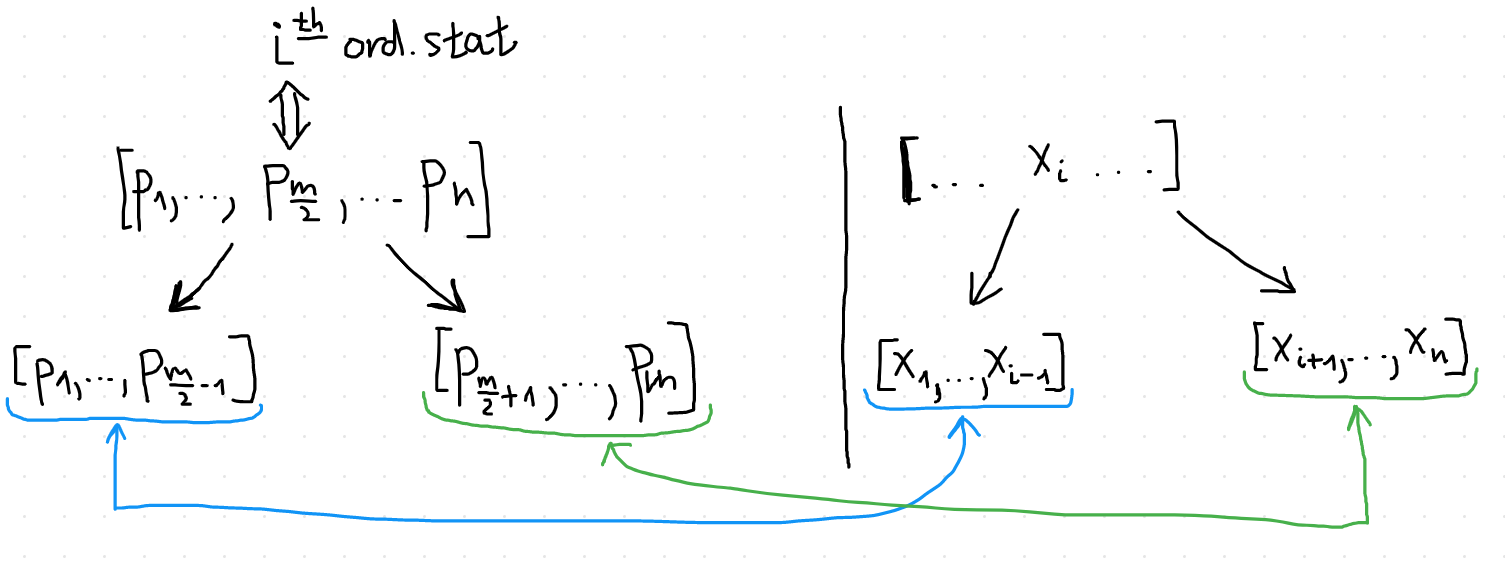
\includegraphics[width=\textwidth]{pics/k_ord_stats.png}
        \caption{Поясняющая картинка.}
    \end{figure}
    \no то есть мы сделаем $\O(\log m)$ вызовов этой процедуры, при этом суммарная длина массивов, в которых ищется статистика $\leq n \Longrightarrow \O(n\log m)$.
    
    Таким образом, мы найдем все нужные статистики. Общая сложность сложится из рекуррентной схемы и первоначальной сортировки массива $[p]$, то есть 
    \begin{equation}
        \O(n\log m + n + m) = \O(n\log m + m).
    \end{equation}
\end{solution}